\documentclass{article}
  \usepackage{amsmath}
  \usepackage{amssymb}
  \usepackage{graphicx}
  \usepackage{float}
  \usepackage{setspace}
  \usepackage{verbatim}
\topmargin=-1.2cm \oddsidemargin=0.1cm \evensidemargin=0.1cm
\textwidth=16 true cm \textheight=23 true cm

\font\euler=EUSM10 \font\eulers=EUSM7

\begin{document}
\title{ECON 3160 Game Theory \\Assignment $5^{\text{th}}$}
\author{{\normalsize Leonard Sheng(SHENG, Hao), 1155035947, via \LaTeX}}
\date{\today}

\maketitle

\def \Pr{{\rm Pr}}

\baselineskip 0.6cm
\begin{description}
    \item[Problem(a):]We construct an example by giving a static game (the pay-off matrix) and an epistemic model for that game.
    \begin{center}
        \begin{tabular}{rrcc}

                   &            & \multicolumn{ 2}{c}{{\bf Barbara}} \\

                   &            &          L &          R \\

        \multicolumn{ 1}{c}{{\bf You}} &          U &      (1,0) &      (1,0) \\

        \multicolumn{ 1}{c}{{\bf }} &          D &      (0,0) &      (0,0) \\

        \end{tabular}

        {\bf Table.1.1 }The static game for {\bf HW5(a)}
    \end{center}


    \begin{center}
              % Table generated by Excel2LaTeX from sheet 'AE'
        \begin{tabular}{cl}
        \hline
        \hline
        \multicolumn{ 1}{c}{{\bf Type}} & $T_1=\left\{t_1\right\}$ \\

        \multicolumn{ 1}{c}{{\bf }} & $T_2=\left\{t_2\right\}$ \\
        \hline
        {\bf Belief of You} & $b_1\left(t_1\right)=\left(L,t_2\right)$ \\
        \hline
        {\bf Belief of Barbara} & $b_2\left(t_2\right)=\left(D,t_1\right)$ \\
        \hline
        \hline
        \end{tabular}

        {\bf Table.1.2 }The epistemic model for {\bf HW5(a)}
    \end{center}
        Obviously, Barbara's type $t_2$ express 2-fold belief in opponent's rationality but not 1-fold.\\
    \item[Problem(b):]We construct an example by giving a dynamic game (a representative graph) and an epistemic model for that game.
    \begin{center}
                    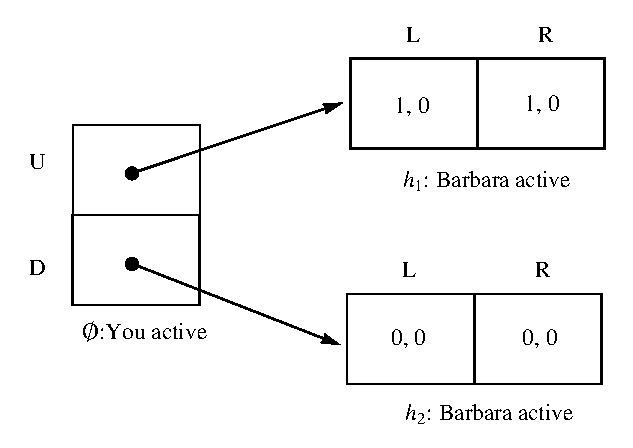
\includegraphics[angle=0, width=0.6\textwidth]{ECON3160A5P1}\\
                    {\bf Figure.1 } Dynamic game for {\bf HW5(b)}
    \end{center}

    \begin{center}
        \begin{tabular}{cl}
        \hline
        \hline
        \multicolumn{ 1}{c}{{\bf Type}} & $T_1=\left\{t_1\right\}$ \\

        \multicolumn{ 1}{c}{{\bf }} & $T_2=\left\{t_2\right\}$ \\
        \hline
        \multicolumn{ 1}{c}{{\bf Belief of You}} & $b_1\left(t_1,\emptyset \right)=\left(L,t_2\right)$ \\
        \hline
        \multicolumn{ 1}{c}{{\bf Belief of Barbara}} & $b_2\left(t_2,h_1\right)=\left(U,t_1\right)$ \\



        \multicolumn{ 1}{c}{{\bf }} & $b_2\left(t_2,h_2\right)=\left(D,t_1\right)$ \\
        \hline
        \hline
        \end{tabular}

        {\bf Table.2.1 }The epistemic model for {\bf HW5(b)}
    \end{center}
     Obviously, Barbara's type $t_2$ express 2-fold belief in opponent's future rationality but not 1-fold.\\
    \item[Problem(c):]9.6. Read my mind\\
    {\bf (a):} \begin{center}
                    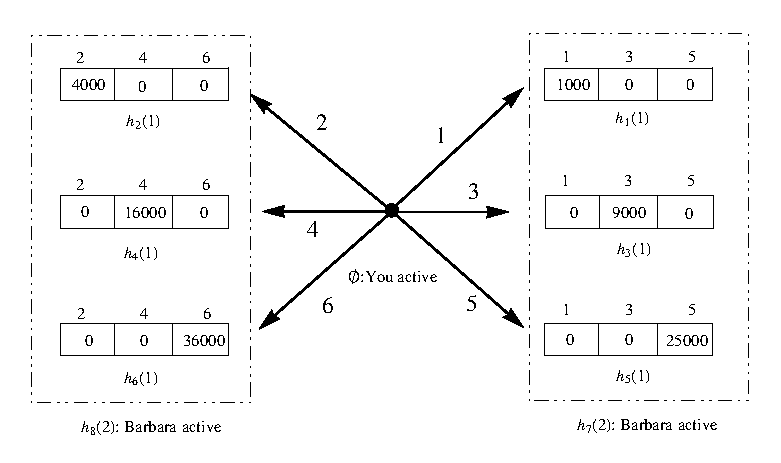
\includegraphics[angle=0, width=0.8\textwidth]{ECON3160A5P3}\\
                    {\bf Figure.3.1 }Dynamic game for {\bf 9.6.Read my mind}
    \end{center}
    \newpage
    {\bf (b):}
    \begin{center}
            % Table generated by Excel2LaTeX from sheet '9.6'
        \begin{tabular}{rrrrrrrrrrr}
        \hline
        \hline
                   &            &                                                                                 \multicolumn{ 9}{c}{{\bf Barbara}} \\

                   &            &  $(1_7,2_8)$ &  $(1_7,4_8)$ &  $(1_7,6_8)$ &  $(3_7,2_8)$ &  $(3_7,4_8)$ &  $(3_7,6_8)$ &  $(5_7,2_8)$ &  $(5_7,4_8)$ &  $(5_7,6_8)$ \\
        \hline
        \multicolumn{ 1}{c}{{\bf You}} &        $1_0$ &       1000 &       1000 &       1000 &          0 &          0 &          0 &          0 &          0 &          0 \\

        \multicolumn{ 1}{c}{{\bf }} &        $3_0$ &          0 &          0 &          0 &       9000 &       9000 &       9000 &          0 &          0 &          0 \\

        \multicolumn{ 1}{c}{{\bf }} &        $5_0$ &          0 &          0 &          0 &          0 &          0 &          0 &      25000 &      25000 &      25000 \\

        \multicolumn{ 1}{c}{{\bf }} &        $2_0$ &       4000 &            &          0 &       4000 &          0 &          0 &       4000 &          0 &          0 \\

        \multicolumn{ 1}{c}{{\bf }} &        $4_0$ &          0 &      16000 &          0 &          0 &      16000 &          0 &          0 &      16000 &          0 \\

        \multicolumn{ 1}{c}{{\bf }} &        $6_0$ &          0 &          0 &      36000 &          0 &          0 &      36000 &          0 &          0 &      36000 \\
        \hline
        \hline
        \end{tabular}

        {\bf Table.3.2.1 }$\Gamma ^0(\emptyset )$: You active, {\bf 9.6.Read my mind}
\end{center}

    \begin{center}
      % Table generated by Excel2LaTeX from sheet '9.6'
        \begin{tabular}{rrrrrrrrrrr}
        \hline
        \hline
                   &            &                                                                                 \multicolumn{ 9}{c}{{\bf Barbara}} \\

                   &            &  $(1_7,2_8)$ &  $(1_7,4_8)$ &  $(1_7,6_8)$ &  $(3_7,2_8)$ &  $(3_7,4_8)$ &  $(3_7,6_8)$ &  $(5_7,2_8)$ &  $(5_7,4_8)$ &  $(5_7,6_8)$ \\
        \hline
        \multicolumn{ 1}{c}{{\bf You}} &        $R_1$ &       1333 &       5333 &      12000 &       1333 &       5333 &      12000 &       1333 &       5333 &      12000 \\

        \multicolumn{ 1}{c}{{\bf }} &        $R_2$ &          0 &          0 &          0 &       4500 &       4500 &       4500 &      12500 &      12500 &      12500 \\

        \multicolumn{ 1}{c}{{\bf }} &        $R_3$ &          0 &      10667 &      12000 &          0 &      10667 &      12000 &          0 &      10667 &      12000 \\
        \hline
        \hline
        \end{tabular}

         {\bf Table.3.2.1B }$\Gamma ^0(\emptyset )$: Some of You randomized strategies, {\bf 9.6.Read my mind}
    \end{center}
      Note: $R_1$, $R_2$ and $R_3$ are randomized strategies:\\
    $R_1=\frac{1}{3}2_0+\frac{1}{3}4_0+\frac{1}{3}6_0$, $R_2=\frac{1}{2}3_0+\frac{1}{2}5_0$, $R_3=\frac{2}{3}4_0+\frac{1}{3}6_0$\\

    \begin{center}
                  % Table generated by Excel2LaTeX from sheet '9.6'
            \begin{tabular}{rrrrrrrrrrr}
            \hline
            \hline
                       &            &                                                                                 \multicolumn{ 9}{c}{{\bf Barbara}} \\

                       &            &  $(1_7,2_8)$ &  $(1_7,4_8)$ &  $(1_7,6_8)$ &  $(3_7,2_8)$ &  $(3_7,4_8)$ &  $(3_7,6_8)$ &  $(5_7,2_8)$ &  $(5_7,4_8)$ &  $(5_7,6_8)$ \\
            \hline
            \multicolumn{ 1}{c}{{\bf You}} &        $1_0$ &       1000 &       1000 &       1000 &          0 &          0 &          0 &          0 &          0 &          0 \\

            \multicolumn{ 1}{c}{{\bf }} &        $3_0$ &          0 &          0 &          0 &       9000 &       9000 &       9000 &          0 &          0 &          0 \\

            \multicolumn{ 1}{c}{{\bf }} &        $5_0$ &          0 &          0 &          0 &          0 &          0 &          0 &      25000 &      25000 &      25000 \\
            \hline
            \hline
            \end{tabular}

         {\bf Table.3.2.2 }$\Gamma ^0(h_7)$: Barbara active, {\bf 9.6.Read my mind}
    \end{center}

    \begin{center}
              % Table generated by Excel2LaTeX from sheet '9.6'
        \begin{tabular}{rrrrrrrrrrr}
        \hline
        \hline
                   &            &                                                                                 \multicolumn{ 9}{c}{{\bf Barbara}} \\

                   &            &  $(1_7,2_8)$ &  $(1_7,4_8)$ &  $(1_7,6_8)$ &  $(3_7,2_8)$ &  $(3_7,4_8)$ &  $(3_7,6_8)$ &  $(5_7,2_8)$ &  $(5_7,4_8)$ &  $(5_7,6_8)$ \\
        \hline
        \multicolumn{ 1}{c}{{\bf You}} &        $2_0$ &       4000 &            &          0 &       4000 &          0 &          0 &       4000 &          0 &          0 \\

        \multicolumn{ 1}{c}{{\bf }} &        $4_0$ &          0 &      16000 &          0 &          0 &      16000 &          0 &          0 &      16000 &          0 \\

        \multicolumn{ 1}{c}{{\bf }} &        $6_0$ &          0 &          0 &      36000 &          0 &          0 &      36000 &          0 &          0 &      36000 \\
        \hline
        \hline
        \end{tabular}

         {\bf Table.3.2.3 }$\Gamma ^0(h_8)$: Barbara active, {\bf 9.6.Read my mind}
    \end{center}
    We begin to use the conditional dominance procedure:
    \newpage
    When the Step.1 is done,
    \begin{center}
              % Table generated by Excel2LaTeX from sheet '9.6AS1'
        \begin{tabular}{rrrrrrrrrrr}
        \hline
        \hline
                   &            &                                                                                 \multicolumn{ 9}{c}{{\bf Barbara}} \\

                   &            &  $(1_7,2_8)$ &  $(1_7,4_8)$ &  $(1_7,6_8)$ &  $(3_7,2_8)$ &  $(3_7,4_8)$ &  $(3_7,6_8)$ &  $(5_7,2_8)$ &  $(5_7,4_8)$ &  $(5_7,6_8)$ \\
        \hline
        \multicolumn{ 1}{c}{{\bf You}} &        $3_0$ &          0 &          0 &          0 &       9000 &       9000 &       9000 &          0 &          0 &          0 \\

        \multicolumn{ 1}{c}{{\bf }} &        $5_0$ &          0 &          0 &          0 &          0 &          0 &          0 &      25000 &      25000 &      25000 \\

        \multicolumn{ 1}{c}{{\bf }} &        $2_0$ &       4000 &            &          0 &       4000 &          0 &          0 &       4000 &          0 &          0 \\

        \multicolumn{ 1}{c}{{\bf }} &        $4_0$ &          0 &      16000 &          0 &          0 &      16000 &          0 &          0 &      16000 &          0 \\

        \multicolumn{ 1}{c}{{\bf }} &        $6_0$ &          0 &          0 &      36000 &          0 &          0 &      36000 &          0 &          0 &      36000 \\
        \hline
        \hline
        \end{tabular}

        {\bf Table.3.2.4 }$\Gamma ^1(\emptyset )$: You active, {\bf 9.6.Read my mind}
    \end{center}

    \begin{center}
              % Table generated by Excel2LaTeX from sheet '9.6AS1'
        \begin{tabular}{rrrrrrrrrrr}
        \hline
        \hline
                   &            &                                                                                 \multicolumn{ 9}{c}{{\bf Barbara}} \\

                   &            &  $(1_7,2_8)$ &  $(1_7,4_8)$ &  $(1_7,6_8)$ &  $(3_7,2_8)$ &  $(3_7,4_8)$ &  $(3_7,6_8)$ &  $(5_7,2_8)$ &  $(5_7,4_8)$ &  $(5_7,6_8)$ \\
        \hline
        \multicolumn{ 1}{c}{{\bf You}} &        $3_0$ &          0 &          0 &          0 &       9000 &       9000 &       9000 &          0 &          0 &          0 \\

        \multicolumn{ 1}{c}{{\bf }} &        $5_0$ &          0 &          0 &          0 &          0 &          0 &          0 &      25000 &      25000 &      25000 \\
        \hline
        \hline
        \end{tabular}

        {\bf Table.3.2.5 }$\Gamma ^1(h_7)$: Barbara active, {\bf 9.6.Read my mind}
    \end{center}

    \begin{center}
              % Table generated by Excel2LaTeX from sheet '9.6AS1'
        \begin{tabular}{rrrrrrrrrrr}
        \hline
        \hline
                   &            &                                                                                 \multicolumn{ 9}{c}{{\bf Barbara}} \\

                   &            &  $(1_7,2_8)$ &  $(1_7,4_8)$ &  $(1_7,6_8)$ &  $(3_7,2_8)$ &  $(3_7,4_8)$ &  $(3_7,6_8)$ &  $(5_7,2_8)$ &  $(5_7,4_8)$ &  $(5_7,6_8)$ \\
        \hline
        \multicolumn{ 1}{c}{{\bf You}} &        $2_0$ &       4000 &            &          0 &       4000 &          0 &          0 &       4000 &          0 &          0 \\

        \multicolumn{ 1}{c}{{\bf }} &        $4_0$ &          0 &      16000 &          0 &          0 &      16000 &          0 &          0 &      16000 &          0 \\

        \multicolumn{ 1}{c}{{\bf }} &        $6_0$ &          0 &          0 &      36000 &          0 &          0 &      36000 &          0 &          0 &      36000 \\
        \hline
        \hline
        \end{tabular}

        {\bf Table.3.2.6 }$\Gamma ^1(h_8)$: Barbara active, {\bf 9.6.Read my mind}
    \end{center}
    \newpage
    When the Step.2 is done,
    \begin{center}
              % Table generated by Excel2LaTeX from sheet '9.6AS2'
        \begin{tabular}{rrrrrrrr}
        \hline
        \hline
                   &            &                                          \multicolumn{ 6}{c}{{\bf Barbara}} \\

                   &            &  $(3_7,2_8)$ &  $(3_7,4_8)$ &  $(3_7,6_8)$ &  $(5_7,2_8)$ &  $(5_7,4_8)$ &  $(5_7,6_8)$ \\
        \hline
        \multicolumn{ 1}{c}{{\bf You}} &        $3_0$ &       9000 &       9000 &       9000 &          0 &          0 &          0 \\

        \multicolumn{ 1}{c}{{\bf }} &        $5_0$ &          0 &          0 &          0 &      25000 &      25000 &      25000 \\

        \multicolumn{ 1}{c}{{\bf }} &        $2_0$ &       4000 &          0 &          0 &       4000 &          0 &          0 \\

        \multicolumn{ 1}{c}{{\bf }} &        $4_0$ &          0 &      16000 &          0 &          0 &      16000 &          0 \\

        \multicolumn{ 1}{c}{{\bf }} &        $6_0$ &          0 &          0 &      36000 &          0 &          0 &      36000 \\
        \hline
        \hline
        \end{tabular}

        {\bf Table.3.2.7 }$\Gamma ^2(\emptyset )$: You active, {\bf 9.6.Read my mind}
    \end{center}

    \begin{center}
              % Table generated by Excel2LaTeX from sheet '9.6AS2'
        \begin{tabular}{rrrrrrrr}
        \hline
        \hline
                   &            &                                          \multicolumn{ 6}{c}{{\bf Barbara}} \\

                   &            &  $(3_7,2_8)$ &  $(3_7,4_8)$ &  $(3_7,6_8)$ &  $(5_7,2_8)$ &  $(5_7,4_8)$ &  $(5_7,6_8)$ \\
        \hline
        \multicolumn{ 1}{c}{{\bf You}} &        $3_0$ &       9000 &       9000 &       9000 &          0 &          0 &          0 \\

        \multicolumn{ 1}{c}{{\bf }} &        $5_0$ &          0 &          0 &          0 &      25000 &      25000 &      25000 \\
        \hline
        \hline
        \end{tabular}

        {\bf Table.3.2.8 }$\Gamma ^2(h_7)$: Barbara active, {\bf 9.6.Read my mind}
    \end{center}

    \begin{center}
              % Table generated by Excel2LaTeX from sheet '9.6AS2'
        \begin{tabular}{rrrrrrrr}
        \hline
        \hline
                   &            &                                          \multicolumn{ 6}{c}{{\bf Barbara}} \\

                   &            &  $(3_7,2_8)$ &  $(3_7,4_8)$ &  $(3_7,6_8)$ &  $(5_7,2_8)$ &  $(5_7,4_8)$ &  $(5_7,6_8)$ \\
        \hline
        \multicolumn{ 1}{c}{{\bf You}} &        $2_0$ &       4000 &          0 &          0 &       4000 &          0 &          0 \\

        \multicolumn{ 1}{c}{{\bf }} &        $4_0$ &          0 &      16000 &          0 &          0 &      16000 &          0 \\

        \multicolumn{ 1}{c}{{\bf }} &        $6_0$ &          0 &          0 &      36000 &          0 &          0 &      36000 \\
        \hline
        \hline
        \end{tabular}

         {\bf Table.3.2.9 }$\Gamma ^2(h_8)$: Barbara active, {\bf 9.6.Read my mind}
    \end{center}
    When the Step.3 is done,
    \begin{center}
              % Table generated by Excel2LaTeX from sheet '9.6AS3'
        \begin{tabular}{rrrrrrrr}
        \hline
        \hline
                   &            &                                          \multicolumn{ 6}{c}{{\bf Barbara}} \\

                   &            &  $(3_7,2_8)$ &  $(3_7,4_8)$ &  $(3_7,6_8)$ &  $(5_7,2_8)$ &  $(5_7,4_8)$ &  $(5_7,6_8)$ \\
        \hline
        \multicolumn{ 1}{c}{{\bf You}} &        $3_0$ &       9000 &       9000 &       9000 &          0 &          0 &          0 \\

        \multicolumn{ 1}{c}{{\bf }} &        $5_0$ &          0 &          0 &          0 &      25000 &      25000 &      25000 \\

        \multicolumn{ 1}{c}{{\bf }} &        $4_0$ &          0 &      16000 &          0 &          0 &      16000 &          0 \\

        \multicolumn{ 1}{c}{{\bf }} &        $6_0$ &          0 &          0 &      36000 &          0 &          0 &      36000 \\
        \hline
        \hline
        \end{tabular}

        {\bf Table.3.2.10 }$\Gamma ^3(\emptyset )$: You active, {\bf 9.6.Read my mind}
    \end{center}

    \begin{center}
              % Table generated by Excel2LaTeX from sheet '9.6AS3'
        \begin{tabular}{rrrrrrrr}
        \hline
        \hline
                   &            &                                          \multicolumn{ 6}{c}{{\bf Barbara}} \\

                   &            &  $(3_7,2_8)$ &  $(3_7,4_8)$ &  $(3_7,6_8)$ &  $(5_7,2_8)$ &  $(5_7,4_8)$ &  $(5_7,6_8)$ \\
        \hline
        \multicolumn{ 1}{c}{{\bf You}} &        $3_0$ &       9000 &       9000 &       9000 &          0 &          0 &          0 \\

        \multicolumn{ 1}{c}{{\bf }} &        $5_0$ &          0 &          0 &          0 &      25000 &      25000 &      25000 \\
        \hline
        \hline
        \end{tabular}

         {\bf Table.3.2.11 }$\Gamma ^3(h_7)$: Barbara active, {\bf 9.6.Read my mind}
    \end{center}

    \begin{center}
              % Table generated by Excel2LaTeX from sheet '9.6AS3'
        \begin{tabular}{rrrrrrrr}
        \hline
        \hline
                   &            &                                          \multicolumn{ 6}{c}{{\bf Barbara}} \\

                   &            &  $(3_7,2_8)$ &  $(3_7,4_8)$ &  $(3_7,6_8)$ &  $(5_7,2_8)$ &  $(5_7,4_8)$ &  $(5_7,6_8)$ \\
        \hline
        \multicolumn{ 1}{c}{{\bf You}} &        $4_0$ &          0 &      16000 &          0 &          0 &      16000 &          0 \\

        \multicolumn{ 1}{c}{{\bf }} &        $6_0$ &          0 &          0 &      36000 &          0 &          0 &      36000 \\
        \hline
        \hline
        \end{tabular}

        {\bf Table.3.2.12 }$\Gamma ^3(h_8)$: Barbara active, {\bf 9.6.Read my mind}
    \end{center}
    ...\\
    ...
    \newpage
    After so many steps (actually 9 of them), we have the final matrix:
    \begin{center}
              % Table generated by Excel2LaTeX from sheet 'S9'
        \begin{tabular}{rrr}
        \hline
        \hline
                   &            & {\bf Barbara} \\

                   &            &  $(5_7,6_8)$ \\
        \hline
         {\bf You} &        $6_0$ &      36000 \\
        \hline
        \hline
        \end{tabular}

        {\bf Table.3.2.13 }$\Gamma ^{\text{*}}(\emptyset )$: You active, {\bf 9.6.Read my mind}
    \end{center}
    \begin{center}
              % Table generated by Excel2LaTeX from sheet 'S9'
        \begin{tabular}{rrr}
        \hline
        \hline
                   &            & {\bf Barbara} \\

                   &            &  $(5_7,6_8)$ \\
        \hline
         {\bf You} &        $5_0$ &      25000 \\
        \hline
        \hline
        \end{tabular}

         {\bf Table.3.2.14 }$\Gamma ^{*}(h_7)$: Barbara active, {\bf 9.6.Read my mind}
    \end{center}
    \begin{center}
              % Table generated by Excel2LaTeX from sheet 'S9'
        \begin{tabular}{rrr}
        \hline
        \hline
                   &            & {\bf Barbara} \\

                   &            &  $(5_7,6_8)$ \\
        \hline
         {\bf You} &        $6_0$ &      36000 \\
        \hline
        \hline
        \end{tabular}

        {\bf Table.3.2.15 }$\Gamma ^{*}(h_8)$: Barbara active, {\bf 9.6.Read my mind}
    \end{center}
    After all, you can rationally pick up $6_0$ under common strong belief in rationality; Barbara can rationally pick up $(5_7,6_8)$ under common strong belief in rationality.\\
    Under common belief in rationality, the possible outcome you deem is that you choose $6_0$, Barbara chooses $(5_7,6_8)$ and both of you and Barbara will get $36000$ euro.\\
    {\bf (c):}
    \begin{itemize}
      \item At first, you find that a randomized strategy $R_1=\frac{1}{3}2_0+\frac{1}{3}4_0+\frac{1}{3}6_0$ will guarantee you at least $\frac{4000}{3}$ which is large than the optimal outcome of strategy $1_0$. You eliminate strategy $1_0$ on the `first day'.
      \item Such reasoning is also noticed by Barbara because she gives you enough benefit of doubt that you are rational. So, if she find herself is at $h_7$, which can only be lead to by your strategies $1_0$, $3_0$ or $5_0$, she will definitely refuse the possibility of $1_0$. If you want to pick up strategy $1_0$ getting into history $h_7$ and take home at most $1000$ euros, why don't you pick up $R_1$ which lead to $h_8$ and give you more euros? So she will never pick the strategy groups that give she the choice $1_7$ at history $h_7$.
      \item Because you are also assume Barbara is rational as long as you can, you recognize in history $h_7$, Barbara will never choice $1_0$. Thus your randomized strategy $R_2=\frac{1}{2}3_0+\frac{1}{2}5_0$ guarantees you at least $4500$ euros, which strictly dominates your strategy $2_0$. You eliminate $2_0$ at initial.
      \item Barbara also recognizes this. Thus, when she find herself at $h_8$, it's her belief you may have chosen $4_0$, $6_0$ or a randomized strategy between them, but never $2_0$. So she will never choose $2_8$ at $h_8$.
      \item You also find that Barbara will never pick up $2_8$ at $h_8$. Thus Your randomized strategy $R_3=\frac{2}{3}4_0+\frac{1}{3}6_0$ guarantees you at least $\frac{32000}{3}$ euros, which strictly dominates your strategy $3_0$. You eliminate $3_0$ at initial.
      \item Barbara finds that the only possibility lead to $h_7$ is that you has chosen $5_0$, as long as both of you reason like above. So she will choose $5_7$ without doubt at $h_7$.
      \item You also find your strategy $5_0$ will lead to $h_7$ will Barbara will pick up $5_7$ without doubt and yield $25000$ euros for both of you, which strictly dominates your strategy $4_0$. You eliminate $4_0$ from the initial.
      \item Barbara finds that the only possibility lead to $h_8$ is that you has chosen $6_0$, as long as both of you reason like above. So she will choose $6_8$ without doubt at $h_8$.
      \item Now your strategy $6_0$ will guarantee you $36000$ euros, which strictly dominates $5_0$. You can eliminate it from the initial. However, once Barbara find herself at $h_7$, she can not assume you are rationally together that you have a type consist with common strong belief of rationality. That's why we cannot eliminate $5_0$ as Barbara's uncertainty from the $h_7$.
    \end{itemize}
    {\bf (f):}Before any elimination, the pay-off for each information set is identical to the Table.3.2.1, Table.3.2.2 and Table.3.2.3 in the part (b). There isn't any strictly dominated strategy groups we can eliminate from $\Gamma ^{0}(h_7)$ and $\Gamma ^{0}(h_8)$. Moreover, Backward elimination doesn't allowed any forward elimination. Thus, we should only focus on the $\Gamma ^{0}(\emptyset )$.
        \begin{center}
              % Table generated by Excel2LaTeX from sheet '9.6AS1'
        \begin{tabular}{rrrrrrrrrrr}
        \hline
        \hline
                   &            &                                                                                 \multicolumn{ 9}{c}{{\bf Barbara}} \\

                   &            &  $(1_7,2_8)$ &  $(1_7,4_8)$ &  $(1_7,6_8)$ &  $(3_7,2_8)$ &  $(3_7,4_8)$ &  $(3_7,6_8)$ &  $(5_7,2_8)$ &  $(5_7,4_8)$ &  $(5_7,6_8)$ \\
        \hline
        \multicolumn{ 1}{c}{{\bf You}} &        $3_0$ &          0 &          0 &          0 &       9000 &       9000 &       9000 &          0 &          0 &          0 \\

        \multicolumn{ 1}{c}{{\bf }} &        $5_0$ &          0 &          0 &          0 &          0 &          0 &          0 &      25000 &      25000 &      25000 \\

        \multicolumn{ 1}{c}{{\bf }} &        $2_0$ &       4000 &            &          0 &       4000 &          0 &          0 &       4000 &          0 &          0 \\

        \multicolumn{ 1}{c}{{\bf }} &        $4_0$ &          0 &      16000 &          0 &          0 &      16000 &          0 &          0 &      16000 &          0 \\

        \multicolumn{ 1}{c}{{\bf }} &        $6_0$ &          0 &          0 &      36000 &          0 &          0 &      36000 &          0 &          0 &      36000 \\
        \hline
        \hline
        \end{tabular}

        {\bf Table.3.2.4 }$\Gamma ^{**}(\emptyset )$: You active, {\bf 9.6.Read my mind}
    \end{center}
    We can only eliminate your strategy $1_0$ from $\Gamma ^{0}(\emptyset )$. Thus, your strategies $3_0$, $5_0$, $2_0$, $4_0$, $6_0$ can be rationally chosen under common belief in future rationality; All of Barbara's strategies can be rationally chosen under common belief in future rationality.\\
    The outcome you deem possible are that you pick up one from \{$3_0$, $5_0$, $2_0$, $4_0$, $6_0$\}, Barbara picks one from \{$(1_7,2_8)$, $(1_7,4_8)$, $(1_7,6_8)$, $(3_7,2_8)$, $(3_7,4_8)$, $(3_7,6_8)$, $(5_7,2_8)$, $(5_7,4_8)$, $(5_7,6_8)$\}  and both of you will get $0$, $4000$, $9000$, $16000$, $25000$, or $36000$ euros according to the matrix above.\\
    Obviously the outcome you deem possible under common strong belief in rationality in part(b) is a subset of the outcome you deem possible under common belief in future rationality, which is consist with {\it THEOREM 9.4.2} in the textbook.
\end{description}
\end{document}
